\section{Week 2}
\subsection{Objective}
For week 2, we are going to regard the \textit{Bayesian Optimal Design} problem for linear regression, and use this to implement a reference implementation, to be used later.
We can then also explore the effect of different data sizes, different priors and the difference between estimating an objective function through sampling versus calculating it analytically.
\subsection{Theory}
\subsubsection{Bayesian Optimal Design}
Often in scientific contexts as well as other cases, one might have a model that one wishes to strengthen in one way or another using experimental data.
Performing the experiments needed to strengthen one's model can be expensive however, so having an efficient strategy to do such can save important ressources.
This is where \textit{Bayesian Optimal Design} comes in.

The Bayesian Optimal Design problem is about finding a design $\B{d}$ from a design space $\B{D}$, that optimizes some kind of utility function.\cite{ryan15} 
For this project, we wish to maximize the expected information gain from the prior to the posterior.
% For this project, that utility function is the mutual information gained from an experiment by measuring at "location" $\B{d}$.\\
To find the optimal design, we want to find a maximizer $\B{d}^*$ defined as such:
\begin{equation}\B{d}^* = \arg \max_{\B{d}\in \B{D}} I(\B{d})\end{equation}
Where $I(\B{d})$ is the \textit{Mutual Information} between the prior and posterior when adjusted for data observed at $\B{d}$.\\
\subsubsection{Mutual Information}
The amount of information of an experiment is often defined as the negative differential entropy defined as such\cite{lindley56}:
\begin{equation}H(X) = \int_{X}p(x)\log p(x)dx\end{equation}
Thus, the information known before $\B{y}$ is observed from $\B{d}$ is
\begin{equation}\label{eq:entropy-prior}H_1 = \int_{\Theta}p(\theta)\log p(\theta)d\theta\end{equation}
and after is
\begin{equation}\label{eq:entropy-posterior}H_2(\B{y}, \B{d}) = \int_{\Theta}p(\theta| \B{y}, \B{d})\log p(\theta| \B{y}, \B{d})d\theta\end{equation}
The gain of information must thus be
\begin{equation}H_\textrm{gain}(\B{y}, \B{d}) = H_2(\B{y}, \B{d}) - H_1\end{equation}
If we instead regard equation \ref{eq:entropy-prior} and \ref{eq:entropy-posterior} as expectations we get
\begin{equation} = \mathbb{E}_\theta[\log p(\theta | \B{y}, \B{d})] - \mathbb{E}_\theta [\log p(\theta )]  = \mathbb{E}_\theta [\log(p(\theta | \B{y}, \B{d})) - \log(p(\theta))]\end{equation}
Before we perform the experiment, we do not know what the outcome will be. Instead, we'll just regard the expected outcome by taking the expectation over $\B{y}$:
\begin{equation} \label{eq:mi}\mathbb{E}_\B{y}[H_\textrm{grain}(\B{y}, \B{d})]  = \mathbb{E}_\B{y}[\mathbb{E}_\theta [\log(p(\theta | \B{y}, \B{d})) - \log(p(\theta))]]\end{equation}
This expression is called the \textit{Mutual Information} between the prior and posterior, and will be denoted $I(\B{d})$.
We can put a new interpretation upon this by expanding equation \ref{eq:mi} using Bayes' rule:
\begin{equation} I(\B{d})  = \mathbb{E}_\B{y}[\mathbb{E}_\theta [\log(p(\B{y} | \B{\theta}, \B{d})) - \log(p(\B{y}|\B{d}))]]\end{equation}
Then we can use that $\frac{p(\B{y}, \B{\theta}|\B{d})}{p(\theta)}=p(\B{y| \theta, \B{d}})$:
\begin{equation} I(\B{d})  = \mathbb{E}_\B{y}[\mathbb{E}_\theta [\log\left(\frac{p(\B{y}, \B{\theta}|\B{d})}{p(\theta)}\right) - \log(p(\B{y}|\B{d}))]] = \mathbb{E}_\B{y}[\mathbb{E}_\theta [\log\left(\frac{p(\B{y}, \B{\theta}|\B{d})}{p(\theta)p(\B{y}|\B{d})}\right)]]\end{equation}
$$ = \textsc{KL}(p(\B{y}, \theta | \B{d})|| p(\theta)p(\B{y}|\B{d}))$$
Two random variables $X$ and $Y$ are said to be \textit{independent} if the product of their distributions is the same as their joint distribution i.e.
\begin{equation}p(X,Y) = p(X)p(Y)\end{equation}
Thus, Mutual Information measures how close the prior and the evidence \todo{check if indeed this is evidence}are to be independent. 
If $\B{d}$ is picked such that the prior has a high probability of being able to predict $\B{y}|\B{d}$, then the mutual information is going to be close to 0. 
If, on the contrary, $\B{d}$ is picked such that the prior has a low probability of being able to predict $\B{y}|\B{d}$, the mutual information is going to be large.
Thus one could expect that an optimizer would prefer to pick a $\B{d}$ within an area where the prior is not very representative of the underlying generating function.
Of course, in an experimental design context we do not have access to this underlying function as we might not be able to simulate experiments accurately. Instead, the expectation expressions in \ref{eq:mi}
makes it such that we only regard the expected information gain for any given underlying function.

\subsubsection{Evaluating the Mutual Information through sampling}
Without using any assumptions about the nature of our model or data, we can utilize Monte Carlo sampling to optain an accurate estimate on the expectations in equation \ref{eq:mi}.
For $N$ samples of $\theta$ and $M$ samples of $\B{y}$ this thus looks like
\begin{equation}
  I(\B{d}) \approx \frac{1}{NM}\sum_{i=0}^N\sum_{j=0}^M(\log (p(\theta_i | \B{y}_j, \B{d})) - \log(p(\theta_i)))
\end{equation}
Picking samples of $\B{y}$ nescessitates that we can simulate the experiment however.
Instead, we will use the reparamerization trick to sample M samples of $\B{z}\in \mathcal{N}(0, \sigma^2_\B{y})$
and then use equation \ref{eq:likelihood-generating} to get samples of $\B{y}$ by
\begin{equation}
  \B{y}_{ij} = \B{d}\theta_i + \B{z}_j
\end{equation}
thus 
\begin{equation}
  I(\B{d}) \approx \frac{1}{NM}\sum_{i=0}^N\sum_{j=0}^M(\log (p(\theta_i | \B{d} \theta_i + \B{z}_j, \B{d})) - \log(p(\theta_i)))
\end{equation}

\subsubsection{Evaluating the Mutual Information through analytical solutions}
It also happens that when we transform equation \ref{eq:mi} using sum of expectations, one can use the known solution to entropy of multivariate normal distributions:
\begin{equation} \mathbb{E}_\B{y}[H_\textrm{grain}(\B{y}, \B{d})]  = \mathbb{E}_\B{y}[\mathbb{E}_\theta [\log(p(\theta | \B{y}, \B{d})) - \log(p(\theta))]]\end{equation}

\subsubsection{old part}
\begin{equation}
= \iint p(\mathbf{x,y})\ln (\frac{p(\mathbf{x,y})}{p(\mathbf{x})p(\mathbf{y})}) \ d\mathbf{x}\ d\mathbf{y}
\end{equation}
Mutual information is defined as
$$I(\B{d}) = \int_{\Theta}\int_{\B{Y}}p(\B{\theta}, \B{y}|\B{d})[\log p(\B{\theta}, \B{y}|\B{d}) - \log p(\B{y}|\B{d}) - \log p(\B{\theta})]d\B{y}d\B{\theta}$$

From last week, we assume that $p(\theta)$ (the prior in our linear model) is normally distributed with mean $\mu_\theta$ and covariance $\Sigma_\theta$.
We can condition $p(\B{\theta}, \B{y}|\B{d})$ on $\B{\theta}$ and get
$$p(\B{\theta}, \B{y}|\B{d}) = p(\B{\theta}|\B{y}, \B{d})p(\B{y}|\B{d})$$
such that 
% Here, $p(\B{\theta}|\B{y}, \B{d})$ is the posterior from last week, which we found also was normally distributed with
% $$\mu_{\B{\theta}| \B{y},\B{d}}=\Sigma_\theta \B{d}^T(\sigma_\B{y} I_N + \B{d}\Sigma_\theta \B{d}^T)^{-1} \B{y}$$
% $$\Sigma_{\B{\theta}| \B{y},\B{d}}=\Sigma_\theta  - \Sigma_\theta\B{d}^T(\sigma_\B{y} I_N + \B{d}\Sigma_\theta \B{d}^T)^{-1} \B{d}\Sigma_\theta$$
% We can then condition the joint distribution $p(\B{\theta}, \B{y}|\B{d})$ on $\B{y}$ and get
% $$p(\B{\theta}, \B{y}|\B{d}) = p(\B{y}|\B{\theta}, \B{d})p(\B{\theta}|\B{d})$$
% Since we know that the parameters of the underlying model are independent on the datapoints that are measured from, we have that $p(\B{\theta} | \B{d})=p(\B{\theta})$. 
% We also have that $p(\B{y}|\B{\theta}, \B{d})$ is the likelihood from last week, 
% which by assumption is normally distributed with mean $\theta^T\B{d}$ and covariance $\sigma_\B{y}^2$.
% Inserting our conditioning into $I(\B{d})$ gives us
% $$I(\B{d})= \int_{\Theta}\int_{\B{Y}}p(\B{y}| \B{\theta},\B{d})p(\theta)[\log p(\B{\theta}| \B{y}, \B{d}) - \log p(\B{\theta})]d\B{y}d\B{\theta}$$
\begin{align*}
  I(\B{d}) &= \int_{\Theta}\int_{\B{Y}}p(\B{\theta}, \B{y}|\B{d})[\log p(\B{\theta}| \B{y}, \B{d}) + \log p(\B{y}|\B{d}) - \log p(\B{y}|\B{d}) - \log p(\B{\theta})]d\B{y}d\B{\theta}\\
 &= \int_{\Theta}\int_{\B{Y}}p(\B{\theta}, \B{y}|\B{d})[\log p(\B{\theta}| \B{y}, \B{d}) - \log p(\B{\theta})]d\B{y}d\B{\theta}\\
 & \mbox{Split integral over $\B{Y}$}\\
 &= \int_{\Theta}\int_{\B{Y}}p(\B{\theta}, \B{y}|\B{d})\log p(\B{\theta}| \B{y}, \B{d}) d\B{y}- \int_{\B{Y}}p(\B{\theta}, \B{y}|\B{d})\log p(\B{\theta})d\B{y}d\B{\theta}\\
 & \mbox{Split joint distribution into conditional and marginal} \\
&= \int_{\Theta}\int_{\B{Y}}p(\B{\theta}, \B{y}|\B{d})\log p(\B{\theta}| \B{y}, \B{d}) d\B{y}- p(\theta)\log p(\B{\theta})\int_{\B{Y}}p(\B{y}|\B{\theta}, \B{d})d\B{y}d\B{\theta}\\
 & \mbox{Use that probability distributions integrate to 1} \\
&= \int_{\Theta}\int_{\B{Y}}p(\B{\theta}, \B{y}|\B{d})\log p(\B{\theta}| \B{y}, \B{d}) d\B{y}- p(\theta)\log p(\B{\theta})d\B{\theta}\\
  & \mbox{Split integral over $\Theta$} \\
&= \int_{\Theta}\int_{\B{Y}}p(\B{\theta}, \B{y}|\B{d})\log p(\B{\theta}| \B{y}, \B{d}) d\B{y}d\B{\theta}- \int_\Theta p(\theta)\log p(\B{\theta})d\B{\theta}\\
  & \mbox{Switch inner integral} \\
&= \int_{\B{Y}}\int_{\B{\Theta}}p(\B{\theta}, \B{y}|\B{d})\log p(\B{\theta}| \B{y}, \B{d}) d\B{\theta}d\B{y}- \int_\Theta p(\theta)\log p(\B{\theta})d\B{\theta}\\
 & \mbox{Split joint distribution into conditional and marginal} \\
&= \int_{\B{Y}}p(\B{y})\int_{\Theta}p(\B{\theta}|\B{y},\B{d})\log p(\B{\theta}| \B{y}, \B{d}) d\B{\theta}d\B{y}- \int_\Theta p(\theta)\log p(\B{\theta})d\B{\theta}\\
& \mbox{Use known integral of entropy (defined as $H(f) = \int_x f(x)\log f(x) dx$) }\\
& \mbox{for multivariate Gaussian distributions, as well as the fact that }\\
& \mbox{the prior and posterior are multivariate Gaussian.} \\
&= \int_{\B{Y}}p(\B{y})\frac{1}{2}\ln \det (2\pi e \Sigma_{\theta|\B{y,d}})d\B{y}- \frac{1}{2}\ln \det (2\pi e\Sigma_\theta)\\
& \mbox{Use that $\Sigma_{\theta | \B{y, d}}$ does not depend on $\B{y}$ (from last week)} \\
& \mbox{and that probability distributions integrate to 1} \\
&= \frac{1}{2}\ln \det (2\pi e \Sigma_{\theta|\B{y,d}})- \frac{1}{2}\ln \det (2\pi e\Sigma_\theta)\\
\end{align*}
\subsubsection{An analytical approach}
\subsection{Design}
The implementation is pretty straight-forward this week, as we only need to implement $I(\textbf{d})$ and plug it in to any out-of-the-box optimizer, such as \texttt{scipy.optimize.minimize(method="BFGS")}.\\
If one implements the optimization using \texttt{autograd.np}, the gradient can also be calculated easily, leading to a more efficient optimization approach.
\subsection{Results}
\begin{figure}
  \centering
  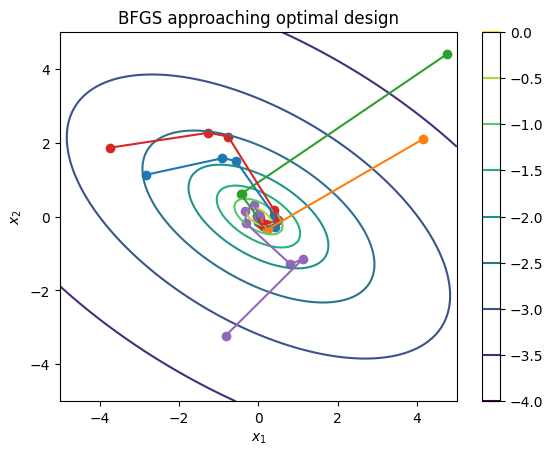
\includegraphics[width=0.8\textwidth]{week2/BFGS.png}
  \caption{BFGS algorithm optimizing for the most mutual information. The contours represent the mutual information.}
  \label{fig:BFGS}
\end{figure}
Running the BFGS algorithm 5 times with random start points over $I(\B{d})$ with $\Sigma_\theta=\begin{bmatrix}7.9 & 3 \\ 4 & 5\end{bmatrix}$ gives the plot seen in Figure \ref{fig:BFGS}. The algorithm usually converges after about 10 steps or so.
\subsection{Evaluation}
As it can be seen in Figure \ref{fig:BFGS}, the algorithm has no problem finding the optimal design for maximizing the mutual information between the prior and the posterior.
